% Options for packages loaded elsewhere
\PassOptionsToPackage{unicode}{hyperref}
\PassOptionsToPackage{hyphens}{url}
\documentclass[
]{article}
\usepackage{xcolor}
\usepackage{amsmath,amssymb}
\setcounter{secnumdepth}{-\maxdimen} % remove section numbering
\usepackage{iftex}
\ifPDFTeX
  \usepackage[T1]{fontenc}
  \usepackage[utf8]{inputenc}
  \usepackage{textcomp} % provide euro and other symbols
\else % if luatex or xetex
  \usepackage{unicode-math} % this also loads fontspec
  \defaultfontfeatures{Scale=MatchLowercase}
  \defaultfontfeatures[\rmfamily]{Ligatures=TeX,Scale=1}
\fi
\usepackage{lmodern}
\ifPDFTeX\else
  % xetex/luatex font selection
\fi
% Use upquote if available, for straight quotes in verbatim environments
\IfFileExists{upquote.sty}{\usepackage{upquote}}{}
\IfFileExists{microtype.sty}{% use microtype if available
  \usepackage[]{microtype}
  \UseMicrotypeSet[protrusion]{basicmath} % disable protrusion for tt fonts
}{}
\makeatletter
\@ifundefined{KOMAClassName}{% if non-KOMA class
  \IfFileExists{parskip.sty}{%
    \usepackage{parskip}
  }{% else
    \setlength{\parindent}{0pt}
    \setlength{\parskip}{6pt plus 2pt minus 1pt}}
}{% if KOMA class
  \KOMAoptions{parskip=half}}
\makeatother
\usepackage{color}
\usepackage{fancyvrb}
\newcommand{\VerbBar}{|}
\newcommand{\VERB}{\Verb[commandchars=\\\{\}]}
\DefineVerbatimEnvironment{Highlighting}{Verbatim}{commandchars=\\\{\}}
% Add ',fontsize=\small' for more characters per line
\newenvironment{Shaded}{}{}
\newcommand{\AlertTok}[1]{\textcolor[rgb]{1.00,0.00,0.00}{\textbf{#1}}}
\newcommand{\AnnotationTok}[1]{\textcolor[rgb]{0.38,0.63,0.69}{\textbf{\textit{#1}}}}
\newcommand{\AttributeTok}[1]{\textcolor[rgb]{0.49,0.56,0.16}{#1}}
\newcommand{\BaseNTok}[1]{\textcolor[rgb]{0.25,0.63,0.44}{#1}}
\newcommand{\BuiltInTok}[1]{\textcolor[rgb]{0.00,0.50,0.00}{#1}}
\newcommand{\CharTok}[1]{\textcolor[rgb]{0.25,0.44,0.63}{#1}}
\newcommand{\CommentTok}[1]{\textcolor[rgb]{0.38,0.63,0.69}{\textit{#1}}}
\newcommand{\CommentVarTok}[1]{\textcolor[rgb]{0.38,0.63,0.69}{\textbf{\textit{#1}}}}
\newcommand{\ConstantTok}[1]{\textcolor[rgb]{0.53,0.00,0.00}{#1}}
\newcommand{\ControlFlowTok}[1]{\textcolor[rgb]{0.00,0.44,0.13}{\textbf{#1}}}
\newcommand{\DataTypeTok}[1]{\textcolor[rgb]{0.56,0.13,0.00}{#1}}
\newcommand{\DecValTok}[1]{\textcolor[rgb]{0.25,0.63,0.44}{#1}}
\newcommand{\DocumentationTok}[1]{\textcolor[rgb]{0.73,0.13,0.13}{\textit{#1}}}
\newcommand{\ErrorTok}[1]{\textcolor[rgb]{1.00,0.00,0.00}{\textbf{#1}}}
\newcommand{\ExtensionTok}[1]{#1}
\newcommand{\FloatTok}[1]{\textcolor[rgb]{0.25,0.63,0.44}{#1}}
\newcommand{\FunctionTok}[1]{\textcolor[rgb]{0.02,0.16,0.49}{#1}}
\newcommand{\ImportTok}[1]{\textcolor[rgb]{0.00,0.50,0.00}{\textbf{#1}}}
\newcommand{\InformationTok}[1]{\textcolor[rgb]{0.38,0.63,0.69}{\textbf{\textit{#1}}}}
\newcommand{\KeywordTok}[1]{\textcolor[rgb]{0.00,0.44,0.13}{\textbf{#1}}}
\newcommand{\NormalTok}[1]{#1}
\newcommand{\OperatorTok}[1]{\textcolor[rgb]{0.40,0.40,0.40}{#1}}
\newcommand{\OtherTok}[1]{\textcolor[rgb]{0.00,0.44,0.13}{#1}}
\newcommand{\PreprocessorTok}[1]{\textcolor[rgb]{0.74,0.48,0.00}{#1}}
\newcommand{\RegionMarkerTok}[1]{#1}
\newcommand{\SpecialCharTok}[1]{\textcolor[rgb]{0.25,0.44,0.63}{#1}}
\newcommand{\SpecialStringTok}[1]{\textcolor[rgb]{0.73,0.40,0.53}{#1}}
\newcommand{\StringTok}[1]{\textcolor[rgb]{0.25,0.44,0.63}{#1}}
\newcommand{\VariableTok}[1]{\textcolor[rgb]{0.10,0.09,0.49}{#1}}
\newcommand{\VerbatimStringTok}[1]{\textcolor[rgb]{0.25,0.44,0.63}{#1}}
\newcommand{\WarningTok}[1]{\textcolor[rgb]{0.38,0.63,0.69}{\textbf{\textit{#1}}}}
\usepackage{longtable,booktabs,array}
\usepackage{calc} % for calculating minipage widths
% Correct order of tables after \paragraph or \subparagraph
\usepackage{etoolbox}
\makeatletter
\patchcmd\longtable{\par}{\if@noskipsec\mbox{}\fi\par}{}{}
\makeatother
% Allow footnotes in longtable head/foot
\IfFileExists{footnotehyper.sty}{\usepackage{footnotehyper}}{\usepackage{footnote}}
\makesavenoteenv{longtable}
\usepackage{graphicx}
\makeatletter
\newsavebox\pandoc@box
\newcommand*\pandocbounded[1]{% scales image to fit in text height/width
  \sbox\pandoc@box{#1}%
  \Gscale@div\@tempa{\textheight}{\dimexpr\ht\pandoc@box+\dp\pandoc@box\relax}%
  \Gscale@div\@tempb{\linewidth}{\wd\pandoc@box}%
  \ifdim\@tempb\p@<\@tempa\p@\let\@tempa\@tempb\fi% select the smaller of both
  \ifdim\@tempa\p@<\p@\scalebox{\@tempa}{\usebox\pandoc@box}%
  \else\usebox{\pandoc@box}%
  \fi%
}
% Set default figure placement to htbp
\def\fps@figure{htbp}
\makeatother
\ifLuaTeX
\usepackage[bidi=basic]{babel}
\else
\usepackage[bidi=default]{babel}
\fi
\babelprovide[main,import]{french}
% get rid of language-specific shorthands (see #6817):
\let\LanguageShortHands\languageshorthands
\def\languageshorthands#1{}
\setlength{\emergencystretch}{3em} % prevent overfull lines
\providecommand{\tightlist}{%
  \setlength{\itemsep}{0pt}\setlength{\parskip}{0pt}}
\usepackage{bookmark}
\IfFileExists{xurl.sty}{\usepackage{xurl}}{} % add URL line breaks if available
\urlstyle{same}
\hypersetup{
  pdftitle={4~ Transformations spectrales -- Traitement d\textquotesingle images satellites avec Python},
  pdflang={fr},
  hidelinks,
  pdfcreator={LaTeX via pandoc}}

\title{4~ Transformations spectrales -- Traitement
d\textquotesingle images satellites avec Python}
\author{}
\date{}

\begin{document}
\maketitle

\phantomsection\label{quarto-document-content}
\phantomsection\label{title-block-header}
\section{\texorpdfstring{\protect\hypertarget{sec-chap03}{}{{4}~
{Transformations
spectrales}}}{4~ Transformations spectrales}}\label{transformations-spectrales}

\subsection{\texorpdfstring{{4.1}
Préambule}{4.1 Préambule}}\label{pruxe9ambule}

Assurez-vous de lire ce préambule avant d'exécutez le reste du notebook.

\subsubsection{\texorpdfstring{{4.1.1}
Objectifs}{4.1.1 Objectifs}}\label{objectifs}

Dans ce chapitre, nous abordons l'exploitation de la dimension spectrale
des images satellites. Ce chapitre est aussi disponible sous la forme
d'un notebook Python:

\href{https://colab.research.google.com/github/sfoucher/TraitementImagesPythonVol1/blob/main/notebooks/03-TransformationSpectrales.ipynb}{\pandocbounded{
\includegraphics[keepaspectratio]{images/colab.png}}}

\subsubsection{\texorpdfstring{{4.1.2}
Librairies}{4.1.2 Librairies}}\label{librairies}

Les librairies qui vont être explorées dans ce chapitre sont les
suivantes:

\begin{itemize}
\item
  \href{https://scipy.org/}{SciPy}
\item
  \href{https://numpy.org/}{NumPy}
\item
  \href{https://github.com/awesome-spectral-indices/spyndex}{spyindex}
\item
  \href{https://rasterio.readthedocs.io/en/stable/}{Rasterio}
\item
  \href{https://docs.xarray.dev/en/stable/}{Xarray}
\item
  \href{https://corteva.github.io/rioxarray/stable/index.html}{rioxarray}
\end{itemize}

Dans l'environnement Google Colab, seul \texttt{rioxarray} doit être
installés:

\phantomsection\label{23b5688b}
\phantomsection\label{cb1}
\begin{Shaded}
\begin{Highlighting}[]
\OperatorTok{\%\%}\NormalTok{capture}
\OperatorTok{!}\NormalTok{pip install }\OperatorTok{{-}}\NormalTok{qU matplotlib rioxarray xrscipy scikit}\OperatorTok{{-}}\NormalTok{image pyarrow spyndex}
\end{Highlighting}
\end{Shaded}

Vérifier les importations:

\phantomsection\label{64a03d08}
\phantomsection\label{cb2}
\begin{Shaded}
\begin{Highlighting}[]
\ImportTok{import}\NormalTok{ numpy }\ImportTok{as}\NormalTok{ np}
\ImportTok{import}\NormalTok{ rioxarray }\ImportTok{as}\NormalTok{ rxr}
\ImportTok{from}\NormalTok{ scipy }\ImportTok{import}\NormalTok{ signal}
\ImportTok{import}\NormalTok{ xarray }\ImportTok{as}\NormalTok{ xr}
\ImportTok{import}\NormalTok{ xrscipy}
\ImportTok{import}\NormalTok{ matplotlib.pyplot }\ImportTok{as}\NormalTok{ plt}
\ImportTok{import}\NormalTok{ spyndex}
\ImportTok{import}\NormalTok{ rasterio }\ImportTok{as}\NormalTok{ rio}
\end{Highlighting}
\end{Shaded}

\subsubsection{\texorpdfstring{{4.1.3} Images
utilisées}{4.1.3 Images utilisées}}\label{images-utilisuxe9es}

Nous allons utilisez les images suivantes dans ce chapitre:

\phantomsection\label{e748f73f}
\phantomsection\label{cb3}
\begin{Shaded}
\begin{Highlighting}[]
\OperatorTok{\%\%}\NormalTok{capture}
\ImportTok{import}\NormalTok{ gdown}

\NormalTok{gdown.download(}\StringTok{\textquotesingle{}https://drive.google.com/uc?export=download\&confirm=pbef\&id=1a6Ypg0g1Oy4AJt9XWKWfnR12NW1XhNg\_\textquotesingle{}}\NormalTok{, output}\OperatorTok{=} \StringTok{\textquotesingle{}RGBNIR\_of\_S2A.tif\textquotesingle{}}\NormalTok{)}
\NormalTok{gdown.download(}\StringTok{\textquotesingle{}https://drive.google.com/uc?export=download\&confirm=pbef\&id=1a6O3L\_abOfU7h94K22At8qtBuLMGErwo\textquotesingle{}}\NormalTok{, output}\OperatorTok{=} \StringTok{\textquotesingle{}sentinel2.tif\textquotesingle{}}\NormalTok{)}
\NormalTok{gdown.download(}\StringTok{\textquotesingle{}https://drive.google.com/uc?export=download\&confirm=pbef\&id=1\_zwCLN{-}x7XJcNHJCH6Z8upEdUXtVtvs1\textquotesingle{}}\NormalTok{, output}\OperatorTok{=} \StringTok{\textquotesingle{}berkeley.jpg\textquotesingle{}}\NormalTok{)}
\NormalTok{gdown.download(}\StringTok{\textquotesingle{}https://drive.google.com/uc?export=download\&confirm=pbef\&id=1dM6IVqjba6GHwTLmI7CpX8GP2z5txUq6\textquotesingle{}}\NormalTok{, output}\OperatorTok{=} \StringTok{\textquotesingle{}SAR.tif\textquotesingle{}}\NormalTok{)}
\NormalTok{gdown.download(}\StringTok{\textquotesingle{}https://drive.google.com/uc?export=download\&confirm=pbef\&id=1aAq7crc\_LoaLC3kG3HkQ6Fv5JfG0mswg\textquotesingle{}}\NormalTok{, output}\OperatorTok{=} \StringTok{\textquotesingle{}carte.tif\textquotesingle{}}\NormalTok{)}
\end{Highlighting}
\end{Shaded}

Vérifiez que vous êtes capable de les lire :

\phantomsection\label{37206eb2}
\phantomsection\label{cb4}
\begin{Shaded}
\begin{Highlighting}[]
\ControlFlowTok{with}\NormalTok{ rxr.open\_rasterio(}\StringTok{\textquotesingle{}berkeley.jpg\textquotesingle{}}\NormalTok{, mask\_and\_scale}\OperatorTok{=} \VariableTok{True}\NormalTok{) }\ImportTok{as}\NormalTok{ img\_rgb:}
    \BuiltInTok{print}\NormalTok{(img\_rgb)}
\ControlFlowTok{with}\NormalTok{ rxr.open\_rasterio(}\StringTok{\textquotesingle{}RGBNIR\_of\_S2A.tif\textquotesingle{}}\NormalTok{, mask\_and\_scale}\OperatorTok{=} \VariableTok{True}\NormalTok{) }\ImportTok{as}\NormalTok{ img\_rgbnir:}
    \BuiltInTok{print}\NormalTok{(img\_rgbnir)}
\ControlFlowTok{with}\NormalTok{ rxr.open\_rasterio(}\StringTok{\textquotesingle{}sentinel2.tif\textquotesingle{}}\NormalTok{, mask\_and\_scale}\OperatorTok{=} \VariableTok{True}\NormalTok{) }\ImportTok{as}\NormalTok{ img\_s2:}
    \BuiltInTok{print}\NormalTok{(img\_s2)}
\ControlFlowTok{with}\NormalTok{ rxr.open\_rasterio(}\StringTok{\textquotesingle{}carte.tif\textquotesingle{}}\NormalTok{, mask\_and\_scale}\OperatorTok{=} \VariableTok{True}\NormalTok{) }\ImportTok{as}\NormalTok{ img\_carte:}
    \BuiltInTok{print}\NormalTok{(img\_carte)}
\end{Highlighting}
\end{Shaded}

\subsection{\texorpdfstring{{4.2} Qu'est ce que l'information
spectrale?}{4.2 Qu'est ce que l'information spectrale?}}\label{quest-ce-que-linformation-spectrale}

L'information spectrale touche à l'exploitation de la dimension
spectrale des images (c.à.d le long des bandes spectrales de l'image).
La taille de cette dimension spectrale dépend du type de capteurs
considéré. Un capteur à très haute résolution spectrale par exemple aura
très peu de bandes (4 ou 5). Un capteur multispectral pourra contenir
une quinzaine de bande. À l'autre extrême, on trouvera les capteurs
hyperspectraux qui peuvent contenir des centaines de bandes spectrales.

\begin{figure}
\centering
\pandocbounded{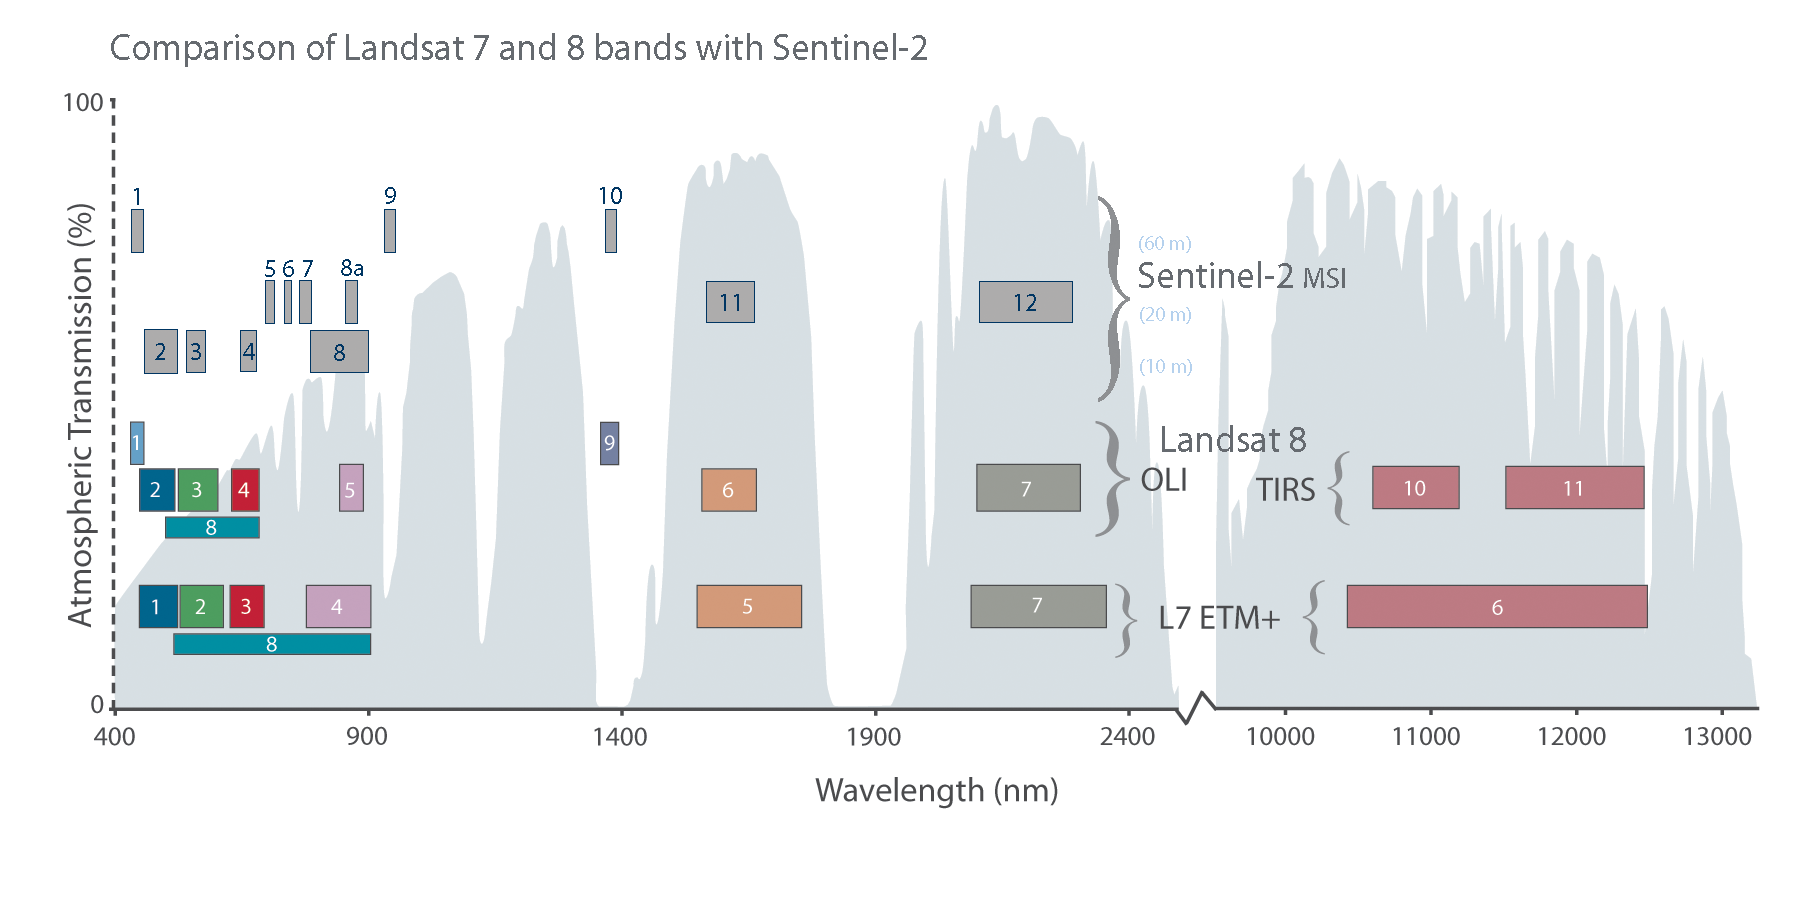
\includegraphics[keepaspectratio]{images/Landsat.v.Sentinel-2-1.png}}
\caption{Positions des bandes spectrales pour quelques capteurs
(\href{https://landsat.gsfc.nasa.gov/article/sentinel-2a-launches-our-compliments-our-complements/}{source})}
\end{figure}

Pour une surface donnée, la forme des valeurs le long de l'axe spectrale
caractérise le type de matériau observé ainsi que son état. On parle
souvent alors de signature spectrale. On peut voir celle-ci comme une
généralisation de la couleur d'un matériau au delà des bandes visibles
du spectre. L'exploitation de ces signatures spectrales est probablement
un des principes les plus importants en télédétection qui le distingue
de la vison par ordinateur.

\subsection{\texorpdfstring{{4.3} Indices
spectraux}{4.3 Indices spectraux}}\label{indices-spectraux}

Il existe une vaste littérature sur les indices spectraux, le choix d'un
indice plutôt qu'un autre dépend fortement de l'application visée, nous
allons simplement couvrir les principes de base ici. Le principe d'un
indice spectral consiste à mettre en valeur certaines caractéristiques
saillantes du spectre comme des pentes, des gradients, etc.

La librairie Python
\href{https://awesome-ee-spectral-indices.readthedocs.io/en/latest/}{Awesome
Spectral Indices} maintient une liste de plus de 200 indices spectraux
(radar et optiques). La liste complète est affichable avec la commande
suivante:

\phantomsection\label{58bacb5c}
\phantomsection\label{cb5}
\begin{Shaded}
\begin{Highlighting}[]
\NormalTok{spyndex.indices}
\end{Highlighting}
\end{Shaded}

\begin{verbatim}
SpectralIndices(['AFRI1600', 'AFRI2100', 'ANDWI', 'ARI', 'ARI2', 'ARVI', 'ATSAVI', 'AVI', 'AWEInsh', 'AWEIsh', 'BAI', 'BAIM', 'BAIS2', 'BCC', 'BI', 'BITM', 'BIXS', 'BLFEI', 'BNDVI', 'BRBA', 'BWDRVI', 'BaI', 'CCI', 'CIG', 'CIRE', 'CRI550', 'CRI700', 'CSI', 'CSIT', 'CVI', 'DBI', 'DBSI', 'DPDD', 'DSI', 'DSWI1', 'DSWI2', 'DSWI3', 'DSWI4', 'DSWI5', 'DVI', 'DVIplus', 'DpRVIHH', 'DpRVIVV', 'EBBI', 'EBI', 'EMBI', 'ENDVI', 'EVI', 'EVI2', 'EVIv', 'ExG', 'ExGR', 'ExR', 'FAI', 'FCVI', 'GARI', 'GBNDVI', 'GCC', 'GDVI', 'GEMI', 'GLI', 'GM1', 'GM2', 'GNDVI', 'GOSAVI', 'GRNDVI', 'GRVI', 'GSAVI', 'GVMI', 'IAVI', 'IBI', 'IKAW', 'IPVI', 'IRECI', 'LSWI', 'MBI', 'MBWI', 'MCARI', 'MCARI1', 'MCARI2', 'MCARI705', 'MCARIOSAVI', 'MCARIOSAVI705', 'MGRVI', 'MIRBI', 'MLSWI26', 'MLSWI27', 'MNDVI', 'MNDWI', 'MNLI', 'MRBVI', 'MSAVI', 'MSI', 'MSR', 'MSR705', 'MTCI', 'MTVI1', 'MTVI2', 'MuWIR', 'NBAI', 'NBLI', 'NBLIOLI', 'NBR', 'NBR2', 'NBRSWIR', 'NBRT1', 'NBRT2', 'NBRT3', 'NBRplus', 'NBSIMS', 'NBUI', 'ND705', 'NDBI', 'NDBaI', 'NDCI', 'NDDI', 'NDGI', 'NDGlaI', 'NDII', 'NDISIb', 'NDISIg', 'NDISImndwi', 'NDISIndwi', 'NDISIr', 'NDMI', 'NDPI', 'NDPolI', 'NDPonI', 'NDREI', 'NDSI', 'NDSII', 'NDSIWV', 'NDSInw', 'NDSWIR', 'NDSaII', 'NDSoI', 'NDTI', 'NDVI', 'NDVI705', 'NDVIMNDWI', 'NDVIT', 'NDWI', 'NDWIns', 'NDYI', 'NGRDI', 'NHFD', 'NIRv', 'NIRvH2', 'NIRvP', 'NLI', 'NMDI', 'NRFIg', 'NRFIr', 'NSDS', 'NSDSI1', 'NSDSI2', 'NSDSI3', 'NSTv1', 'NSTv2', 'NWI', 'NormG', 'NormNIR', 'NormR', 'OCVI', 'OSAVI', 'OSI', 'PI', 'PISI', 'PSRI', 'QpRVI', 'RCC', 'RDVI', 'REDSI', 'RENDVI', 'RFDI', 'RGBVI', 'RGRI', 'RI', 'RI4XS', 'RNDVI', 'RVI', 'S2REP', 'S2WI', 'S3', 'SARVI', 'SAVI', 'SAVI2', 'SAVIT', 'SEVI', 'SI', 'SIPI', 'SLAVI', 'SR', 'SR2', 'SR3', 'SR555', 'SR705', 'SWI', 'SWM', 'SeLI', 'TCARI', 'TCARIOSAVI', 'TCARIOSAVI705', 'TCI', 'TDVI', 'TGI', 'TRRVI', 'TSAVI', 'TTVI', 'TVI', 'TWI', 'TriVI', 'UI', 'VARI', 'VARI700', 'VDDPI', 'VHVVD', 'VHVVP', 'VHVVR', 'VI6T', 'VI700', 'VIBI', 'VIG', 'VVVHD', 'VVVHR', 'VVVHS', 'VgNIRBI', 'VrNIRBI', 'WDRVI', 'WDVI', 'WI1', 'WI2', 'WI2015', 'WRI', 'bNIRv', 'kEVI', 'kIPVI', 'kNDVI', 'kRVI', 'kVARI', 'mND705', 'mSR705', 'sNIRvLSWI', 'sNIRvNDPI', 'sNIRvNDVILSWIP', 'sNIRvNDVILSWIS', 'sNIRvSWIR'])
\end{verbatim}

Le détail d'un indice particulier, par exemple le `NDVI`, est aussi
affichable:

\phantomsection\label{aeaea7e3}
\phantomsection\label{cb7}
\begin{Shaded}
\begin{Highlighting}[]
\NormalTok{spyndex.indices[}\StringTok{"NDVI"}\NormalTok{]}
\end{Highlighting}
\end{Shaded}

\begin{verbatim}
SpectralIndex(NDVI: Normalized Difference Vegetation Index)
        * Application Domain: vegetation
        * Bands/Parameters: ['N', 'R']
        * Formula: (N-R)/(N+R)
        * Reference: https://ntrs.nasa.gov/citations/19740022614
        
\end{verbatim}

\texttt{spyndex} pré-suppose une nomenclature prédéfinie des
\href{https://awesome-ee-spectral-indices.readthedocs.io/en/latest/\#expressions}{bandes},
on peut voir la correspondance sur le tableau ci-dessous:

\phantomsection\label{6adfad8e}
\phantomsection\label{cb9}
\begin{Shaded}
\begin{Highlighting}[]
\NormalTok{spyndex.bands}
\end{Highlighting}
\end{Shaded}

\begin{verbatim}
Bands(['A', 'B', 'G', 'G1', 'N', 'N2', 'R', 'RE1', 'RE2', 'RE3', 'S1', 'S2', 'T', 'T1', 'T2', 'WV', 'Y'])
\end{verbatim}

\begin{longtable}[]{@{}llll@{}}
\caption{Noms des bandes Sentinel-2}\tabularnewline
\toprule\noalign{}
Index & Noms & Spyndex & Noms \\
\midrule\noalign{}
\endfirsthead
\toprule\noalign{}
Index & Noms & Spyndex & Noms \\
\midrule\noalign{}
\endhead
\bottomrule\noalign{}
\endlastfoot
1 & B01 & A & Aérosol \\
2 & B02 & B & Bleu \\
3 & B03 & G & Vert \\
4 & B04 & R & Rouge \\
5 & B05 & RE1 & Red edge 1 \\
6 & B06 & RE1 & Red edge 2 \\
7 & B07 & RE2 & Red edge 3 \\
8 & B08 & N & Proche-infrarouge 1 \\
9 & B08A & N2 & Proche-infrarouge 2 \\
10 & B09 & - & Vapeur d'eau \\
11 & B11 & S1 & Infra-rouge onde courte 1 \\
12 & B12 & S2 & Infra-rouge onde courte 1 \\
\end{longtable}

Deux options sont possibles, on peut soit renommer les noms des bandes
avec \texttt{xarray} ou ``mapper'' les noms vers les noms appropriés.
Regardons les dimensions de notre jeux de données:

\phantomsection\label{aae31d76}
\phantomsection\label{cb11}
\begin{Shaded}
\begin{Highlighting}[]
\NormalTok{img\_s2.dims}
\end{Highlighting}
\end{Shaded}

\begin{verbatim}
('band', 'y', 'x')
\end{verbatim}

On peut simplement changer les index (\texttt{coords}) de la dimension
\texttt{band}:

\phantomsection\label{c7dde0f8}
\phantomsection\label{cb13}
\begin{Shaded}
\begin{Highlighting}[]
\NormalTok{img\_s2 }\OperatorTok{=}\NormalTok{ img\_s2.sel(band }\OperatorTok{=} \BuiltInTok{list}\NormalTok{(}\BuiltInTok{range}\NormalTok{(}\DecValTok{1}\NormalTok{,}\DecValTok{13}\NormalTok{))).assign\_coords(\{}\StringTok{\textquotesingle{}band\textquotesingle{}}\NormalTok{:[}\StringTok{"A"}\NormalTok{, }\StringTok{"B"}\NormalTok{, }\StringTok{"G"}\NormalTok{, }\StringTok{"R"}\NormalTok{, }\StringTok{"RE1"}\NormalTok{, }\StringTok{"RE2"}\NormalTok{, }\StringTok{"RE3"}\NormalTok{, }\StringTok{"N"}\NormalTok{, }\StringTok{"N2"}\NormalTok{, }\StringTok{"WV"}\NormalTok{, }\StringTok{"S1"}\NormalTok{, }\StringTok{"S2"}\NormalTok{]\})}
\NormalTok{img\_s2}\OperatorTok{=}\NormalTok{img\_s2}\OperatorTok{/}\DecValTok{10000} \CommentTok{\# normalisation en réflectance}
\end{Highlighting}
\end{Shaded}

\phantomsection\label{d5e8fa69}
\phantomsection\label{cb14}
\begin{Shaded}
\begin{Highlighting}[]
\ImportTok{from}\NormalTok{ rasterio }\ImportTok{import}\NormalTok{ plot}
\NormalTok{idx }\OperatorTok{=}\NormalTok{ spyndex.computeIndex(}
\NormalTok{    index }\OperatorTok{=}\NormalTok{ [}\StringTok{"NDVI"}\NormalTok{,}\StringTok{"GNDVI"}\NormalTok{,}\StringTok{"SAVI"}\NormalTok{],}
\NormalTok{    params }\OperatorTok{=}\NormalTok{ \{}
        \StringTok{"N"}\NormalTok{: img\_s2.sel(band }\OperatorTok{=} \StringTok{"N"}\NormalTok{),}
        \StringTok{"R"}\NormalTok{: img\_s2.sel(band }\OperatorTok{=} \StringTok{"R"}\NormalTok{),}
        \StringTok{"G"}\NormalTok{: img\_s2.sel(band }\OperatorTok{=} \StringTok{"G"}\NormalTok{),}
        \StringTok{"L"}\NormalTok{: }\FloatTok{0.5}
\NormalTok{    \}}
\NormalTok{)}

\CommentTok{\# Plot the indices (and the RGB image for comparison)}
\NormalTok{fig, ax }\OperatorTok{=}\NormalTok{ plt.subplots(}\DecValTok{2}\NormalTok{,}\DecValTok{2}\NormalTok{,figsize }\OperatorTok{=}\NormalTok{ (}\DecValTok{9}\NormalTok{,}\DecValTok{9}\NormalTok{))}
\NormalTok{[a.axis(}\StringTok{\textquotesingle{}off\textquotesingle{}}\NormalTok{) }\ControlFlowTok{for}\NormalTok{ a }\KeywordTok{in}\NormalTok{ ax.flatten()]}
\NormalTok{plot.show(img\_s2.sel(band }\OperatorTok{=}\NormalTok{ [}\StringTok{"R"}\NormalTok{,}\StringTok{"G"}\NormalTok{,}\StringTok{"B"}\NormalTok{]).data }\OperatorTok{/} \FloatTok{0.3}\NormalTok{,ax }\OperatorTok{=}\NormalTok{ ax[}\DecValTok{0}\NormalTok{,}\DecValTok{0}\NormalTok{],title }\OperatorTok{=} \StringTok{"RGB"}\NormalTok{)}
\NormalTok{plot.show(idx.sel(index }\OperatorTok{=} \StringTok{"NDVI"}\NormalTok{),ax }\OperatorTok{=}\NormalTok{ ax[}\DecValTok{0}\NormalTok{,}\DecValTok{1}\NormalTok{],title }\OperatorTok{=} \StringTok{"NDVI"}\NormalTok{)}
\NormalTok{plot.show(idx.sel(index }\OperatorTok{=} \StringTok{"GNDVI"}\NormalTok{),ax }\OperatorTok{=}\NormalTok{ ax[}\DecValTok{1}\NormalTok{,}\DecValTok{0}\NormalTok{],title }\OperatorTok{=} \StringTok{"GNDVI"}\NormalTok{)}
\NormalTok{plot.show(idx.sel(index }\OperatorTok{=} \StringTok{"SAVI"}\NormalTok{),ax }\OperatorTok{=}\NormalTok{ ax[}\DecValTok{1}\NormalTok{,}\DecValTok{1}\NormalTok{],title }\OperatorTok{=} \StringTok{"SAVI"}\NormalTok{)}
\end{Highlighting}
\end{Shaded}

\begin{figure}
\centering
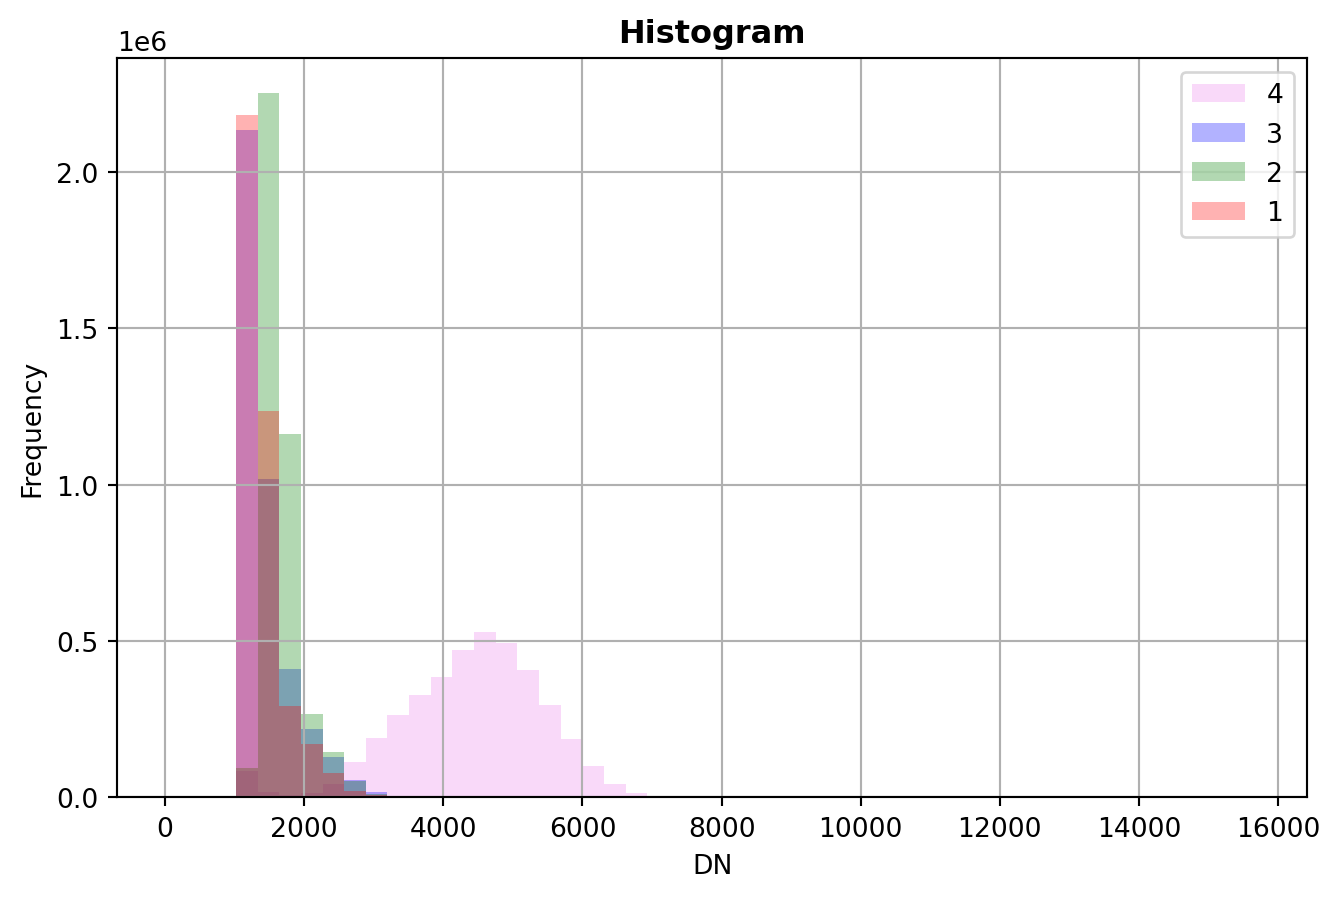
\includegraphics[width=7.46875in,height=7.41667in]{03-TransformationSpectrales_files/figure-html/cell-12-output-1.png}
\caption{}
\end{figure}

On peut vérifier l'utilité des indices en vérifiant leur séparabilité
pour certaines classes d'intérêts. Nous reprenons ici l'exemple de la
section \href{05-ClassificationsSupervisees.html\#sec-05.02.02}{{Section
6.2.3}} pour vérifier l'utilité des indices \texttt{NDVI}, \texttt{NDWI}
et \texttt{NDBI}:

\phantomsection\label{06d714fe}
\phantomsection\label{cb15}
\begin{Shaded}
\begin{Highlighting}[]
\ImportTok{import}\NormalTok{ pandas }\ImportTok{as}\NormalTok{ pd}
\ImportTok{import}\NormalTok{ seaborn }\ImportTok{as}\NormalTok{ sns}

\CommentTok{\# On sélectionne trois classes}
\NormalTok{class\_selected}\OperatorTok{=}\NormalTok{ [}\DecValTok{1}\NormalTok{,}\DecValTok{3}\NormalTok{,}\DecValTok{9}\NormalTok{]}
\NormalTok{df}\OperatorTok{=}\NormalTok{ pd.concat([gdf[gdf[}\StringTok{\textquotesingle{}class\textquotesingle{}}\NormalTok{] }\OperatorTok{==}\NormalTok{c] }\ControlFlowTok{for}\NormalTok{ c }\KeywordTok{in}\NormalTok{ class\_selected], ignore\_index}\OperatorTok{=}\VariableTok{True}\NormalTok{)}
\NormalTok{idx[}\StringTok{"Land Cover"}\NormalTok{] }\OperatorTok{=}\NormalTok{ [nom\_classes[l] }\ControlFlowTok{for}\NormalTok{ l }\KeywordTok{in}\NormalTok{ df[}\StringTok{"class"}\NormalTok{].tolist()]}
\CommentTok{\# Compute the desired spectral indices}
\NormalTok{idx }\OperatorTok{=}\NormalTok{ spyndex.computeIndex(}
\NormalTok{    index }\OperatorTok{=}\NormalTok{ [}\StringTok{"NDVI"}\NormalTok{,}\StringTok{"NDWI"}\NormalTok{,}\StringTok{"NDBI"}\NormalTok{],}
\NormalTok{    params }\OperatorTok{=}\NormalTok{ \{}
        \StringTok{"N"}\NormalTok{: df[}\StringTok{"SR\_B8"}\NormalTok{],}
        \StringTok{"R"}\NormalTok{: df[}\StringTok{"SR\_B4"}\NormalTok{],}
        \StringTok{"G"}\NormalTok{: df[}\StringTok{"SR\_B3"}\NormalTok{],}
        \StringTok{"S1"}\NormalTok{: df[}\StringTok{"SR\_B11"}\NormalTok{]}
\NormalTok{    \}}
\NormalTok{)}

\NormalTok{colors}\OperatorTok{=}\NormalTok{ [couleurs\_classes[c] }\ControlFlowTok{for}\NormalTok{ c }\KeywordTok{in}\NormalTok{ class\_selected]}
\CommentTok{\# Plot a pairplot to check the indices behaviour}
\NormalTok{plt.figure(figsize }\OperatorTok{=}\NormalTok{ (}\DecValTok{15}\NormalTok{,}\DecValTok{15}\NormalTok{))}
\NormalTok{g }\OperatorTok{=}\NormalTok{ sns.PairGrid(idx,hue }\OperatorTok{=} \StringTok{"Land Cover"}\NormalTok{,palette }\OperatorTok{=}\NormalTok{ sns.color\_palette(colors))}
\NormalTok{g.map\_lower(sns.scatterplot)}
\NormalTok{g.map\_upper(sns.kdeplot,fill }\OperatorTok{=} \VariableTok{True}\NormalTok{,alpha }\OperatorTok{=} \FloatTok{.5}\NormalTok{)}
\NormalTok{g.map\_diag(sns.kdeplot,fill }\OperatorTok{=} \VariableTok{True}\NormalTok{)}
\NormalTok{g.add\_legend()}
\NormalTok{plt.show()}
\end{Highlighting}
\end{Shaded}

\begin{figure}
\centering
\pandocbounded{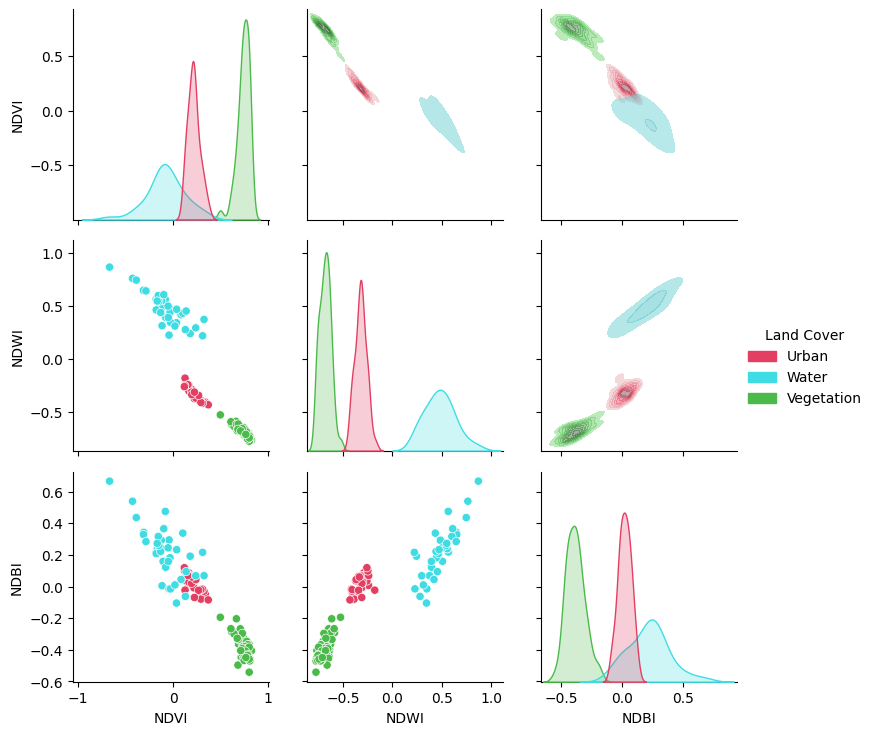
\includegraphics[keepaspectratio]{images/fig-classes-indices.png}}
\caption{Visualisation des points d'une image Sentinel-2 pour trois
classes}
\end{figure}

\end{document}
